\documentclass[a4paper,twoside]{tufte-book} %style file is in the same folder.

\usepackage{color}
\usepackage{xcolor}
\usepackage{framed}
\usepackage{listings}

\usepackage{graphicx}

\usepackage{multicol}              
\usepackage{multirow}
\usepackage{booktabs}
%\usepackage{natbib} 

\usepackage[]{hyperref}
\definecolor{darkblue}{rgb}{0,0,.5}
\hypersetup{colorlinks=true, breaklinks=true, linkcolor=darkblue, menucolor=darkblue, urlcolor=blue, citecolor=darkblue}

\lstset{ % settings for listings needs to be be changed to R sytanx 
language=R,
breaklines = true,
breakautoindent = false,
basicstyle=\ttfamily \scriptsize,
keywordstyle=\color{black},                          
identifierstyle=\color{black},
commentstyle=\color{gray},
frame=single,
framerule=0.4pt,
framesep=3pt,
xleftmargin=3.4pt,
xrightmargin=3.4pt,
numbers=none
}

\setcounter{secnumdepth}{1}


\title{A crash course in\\statistics and R}
\author{Florian Hartig}


\begin{document}
\let\cleardoublepage\clearpage % No empty pages between chapters
\maketitle
\newpage
\tableofcontents

\chapter{Synopsis and Introduction} % Use chapters instead of sections

The purpose of this document is to give a short and concise introduction to the type of statistical analysis most likely to be encountered in elementary experimental and observation setups. It is a crash-course and not meant to replace an proper introductory textbook. For beginners, I recommend \citep{Dormann-ParametrischeStatistik-2013} for German speakers (ebook free of charge for students from Freiburg, contact me) and \citep{Gotelli-PrimerEcologicalStatistics-2004} for English speakers. Also, see the stats help website of our department \href{http://biometry.github.io/APES/}{here}.
 
\chapter{The R environment for statistical computing}

The time where people did statistics with pen, paper and a calculator are over. Statistical analysis nowadays happens on the computer, and a number of software environments exist to do so. In the ecological sciences, R is the de-facto standard for statistical analysis. R is open-source, free, and has a very larger user base, specially in the environmental sciences, that contribute packages for specialized ecological and environmental analysis. Therefore, while maybe not as user-friendly as other software options in every respect, there is practically no way around R.

R is script-based language, which means that you communicate with the computer not by clicking on buttons, but by writing commands either directly in the R console, or first in a text file and then sending it to the R console, which is then evaluating your commands. If you aren't used to this kind of approach yet, it may take a short while to get used to this, but once you are used to it, you will notice how advantageous it is to have all steps of your analysis listed in a text file, being able to repeat everything at any moment. In the rest of this course, we will use R where we need a computer, but I will give no further introduction to R. If you need one, follow  \href{http://biometry.github.io/APES/R/R10-gettingStarted.html}{this link} for an introduction, in including help on how to install the software.

\chapter{Foundational ideas of statistical inference}

When we start discussing statistics, it's tempting to jump right into distributions, models and how to put them in the computer. We'll get to this, but I want to take on step back and discuss the aims of why we want to do statistics, and what we want to get out of it. 

In a nutshell, a statistical analysis consists of 3 parts: the data, a statistical model, and an inferential method. 

\section{The data}

We will speak about how to create data (design of experiments) in a later chapter. For the moment, however, let us assume that we have some data. Usually, this data will contain one variable on which we want to focus. \marginnote{The response variable is the variable for which we try to understand how it responds to other factors.} We call this variable the response variable (sometimes also the depended variable or outcome variable), because we are interested if and how this variable of interest varies (responds, depends) when something else changes. Something else could be an environmental factor (e.g. temperature), it could be an experimental treatment (fertilized vs. non fertilized), or anything else. \marginnote{The predictor variables are those that affect the response.} Those other variables that affect our response are called predictor variables (and also explanatory variables, covariates or independent variables). 

The most common case is that the response variable is a single value, and we will concentrate on this case here. However, there are cases when the response has more than one dimension, or when we are interested in the change of several response variables at a time. {If the response has several dimensions, we have to use multivariate analysis methods, which are not explained here.} The analysis of such data is known as multivariate statistics. We will not cover this here, but if you need it some further links are \href{http://biometry.github.io/APES/Stats/stats50-MultivariateStatistics.html}{here}.

Another important distinction is the type of variables that. Independent of whether we are speaking about the response or the predictor, we distinguish: \marginnote{Variables can be continous, discrete or categorical. Categorical variables can be ordered, unordered, or binary.}

\begin{itemize}
\item Continuous numeric variables (ordered and dense), e.g. temperature
\item Discrete numeric variables (ordered, but discrete), e.g. count data
\item Categorical variables (e.g. a fixed set of options such as red, green blue), which can further be divided into
\begin{itemize}
\item Unordered categorical variables (Nominal) such as red, green, blue 
\item Binary (Dichotomous) variables (dead / survived)
\item Ordered categorical variables (small, medium, large)
\end{itemize}
\end{itemize}

Experience shows that there is certain tendency of beginners to use categorical variables for things that are actually continuous, e.g. by coding body weight of animals into light, medium, heavy. \marginnote{Don't use categorical variables for things that can also be recorded numerically! } The justification stated is often that this avoids the measurement uncertainty. In short: it doesn't, it just creates more problems. Don't use categorical variables for things that can also be recorded numerically! 


\section{Statistical models}

The problem with giving a straight answer to the question of whether the response variable is affected by the predictors is that all our ecological data contains random variability. If we take two pots and plant a plant in each one of them, and we expose one plant to classical music and the other to heavy metal, probably one of them will grow taller. But are we sure that this is an effect of the music, or could it just be due to the fact that no plant is exactly the same, and therefore one of the two must grow taller just by chance?

Thus, to arrive at robust conclusions, we have to make some assumptions about how the growth of plants varies, so that we can see if some differences that we are seeing could be the result of random variation only. These assumptions are what we call a statistical model. \marginnote{A statistical model describes the potential dependence of response on the predictors, as well as random variance in the variables} A statistical model could, for example, make the assumptions that there is a mean growth rate for each classical and heavy metal music, but that the growth of each individual plant varies with a certain distribution around the mean growth of its respective group. Based on this model, we can now ask ourselves (or the computer) certain questions, e.g. for our example whether the data is consistent with the hypothesis that there is no difference between the growth of plants that differ only in the music that they are exposed to.


\section{Inferential methods and their outputs}

The process of and the methods for asking this question, i.e. for using a statistical model and data to draw certain conclusions is called statistical inference. \marginnote{Statistical inference is drawing conclusions from observations using statistical methods}. There are two main inferential procedures. In standard statistics, there are two main inferential procedures that are applied in all kind of settings and models, and the outputs of these two procedures are: p-values and parameter estimates. There is a third option which I will mention very shortly at the end.  

\subsection{p-values}

The use of p-values is connected to the inferential method of null hypothesis significance testing (NHST). The idea is the following: if we have some data observed, and we have a statistical model, we can use this statistical model to specify a fixed hypothesis about how the data did arise. For the example with the plants and music, this hypothesis could be: music has no influence on plants, all differences we see are due to random variation between individuals. Such a scenario is called the null hypothesis. \marginnote{A null hypothesis $H_0$ is a fixed scenario that makes predictions about the expected probabilities of different observations.} Although it is very typical to use the assumption of no effect as null-hypothesis, note that it is really your choice, and you could use anything as null hypothesis, also the assumption: "classical music doubles the growth of plants". The fact that it's the analyst's choice what to fix as null hypothesis is part of the reason why there are are a large number of tests available. We will see a few of them in the following chapter about important hypothesis tests.

If we have a null hypothesis, we calculate the probability that we would see the observed data or data more extreme under this scenario. This allows us to test whether our null hypothesis is compatible wit the data, and thus called a hypothesis tests. We call the probability to see the data or more extreme the p-value. \marginnote{The p-value is the probability to see the data or more extreme data under the null-hypothesis.} If the p-value falls under a certain level (the significance level $\alpha$) we say the null hypothesis was rejected, and there is significant support for the alternative hypothesis. The level of $\alpha$ is a convention, in ecology we chose typically 0.05, so if a p-value falls below 0.05, we can reject the null hypothesis. \marginnote{if p<0.05, we say we have significant evidence to reject the null-hypothesis.} 

A problem with hypothesis tests and p-values is that their results are notoriously misinterpreted. The p-value is NOT the probability that the null hypothesis is true, or the probability that the alternative hypothesis is false, although many authors have made the mistake of interpreting it like that \citep[][]{Cohen-earthisround-1994}. Rather, the idea of p-values is to control the rate of false positives (Type I error). When doing hypothesis tests on random data, with an $\alpha$ level of 0.05, one will get exactly 5\% false positives. Not more and not less.  

\subsection{Parameter estimates}

The second type of output that is reported by most statistical methods are parameter estimates. Without going into too much detail: while the p-value is the probability of the data or more extreme data under a fixed (null) hypothesis, a parameter estimate (often also called point estimate or maximum likelihood estimate) refers to those of many possible hypothesis that are spanned by a parameter that has the highest probability to produce the observed data. 

In plain words, the parameter estimate is our best estimate for a difference between groups, or the influence between parameters. Again, in contrast, the p-value typically tells us the probability that we would see the data if there is no such influence. 

Parameter estimates are typically accompanies by confidence intervals. Sloppily you can think of the 95\% confidence interval of a parameter as the probable range for this area. Somewhat confusing for many, it's not the interval in which the true parameter lies with 95\% probability. Rather, in a repeated experiments, the standard 95\% CI will contain the true value in 95\% of all cases. It's a subtle, but important difference. However, for now, don't worry about it. The CI interval is roughly where we expect the parameter. 

\subsection{Bayesian estimates}

Just for completeness - there are some advanced methods that report a different thing than p-values and the parameter estimates discussed before. Bayesian methods calculate a quantity that is called the posterior parameter estimate. It is similar, but not identical to the parameter estimates discussed previously. You won't need this here, but if you want to know more about those, have a look at \citep{Gelman-BayesianDataAnalysis-2003}.


\chapter{Important hypothesis tests}

After having discussed the concept of hypothesis tests (which produce p-values against a null-hypothesis) and parameter estimates (which produce best estimates and confidence intervals), lets move to practice and get to know the two probably most applied hypothesis tests, the t-test and ANOVA.

\section{t-test}

A t-test tests for differences between the means of two normally distributed samples; or if there is only one sample, between 0 and the mean of the sample. Classifying our variables, we would say the response variable in continuous, and the predictor is categorical (group 1 or group 2), or, if there is only one group, there is no predictor. Again, the statistical model underlying is that of a normally distributed response, and the null hypothesis is that that there is no difference in the mean of the this normal distribution for the two groups, respectively that the sample mean is 0 if we have one group. Depending on the software used, there are usually a number of adjustments possible, e.g. relaxing the assumption that the two groups have the same variance. An example in R, using the classical data from Student (1908) The probable error of the mean. Biometrika, 6, 20. The data which show the effect of two soporific drugs (increase in hours of sleep compared to control) on 10 patients. 

\begin{figure}[htbp]
\begin{center}
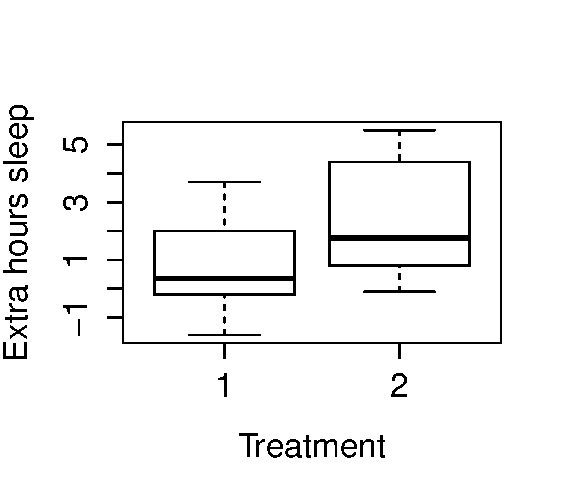
\includegraphics[width=5cm]{ttest}
\caption{Data from Student (1908) The probable error of the mean. Biometrika, 6, 20}
\label{fig: Student Sleep Data}
\end{center}
\end{figure}


\begin{lstlisting}
## Traditional interface
with(sleep, t.test(sleep$extra[sleep$group == 1], extra[group == 2]))
## Formula interface
t.test(extra ~ group, data = sleep)

# Welch Two Sample t-test
# 
# data:  extra by group
# t = -1.8608, df = 17.776, p-value = 0.07939
# alternative hypothesis: true difference in means is not equal to 0
# 95 percent confidence interval:
#   -3.3654832  0.2054832
# sample estimates:
#   mean in group 1 mean in group 2 
# 0.75            2.33 
\end{lstlisting}

Note that the output give a p-value, but also contains the estimates of the means, together with the confidence intervals. 

Suggestion for reporting: p>0.05: differences between groups were not significant. p<0.05: we found a difference of X +- Confidence interval between the groups (p-value for difference from a t-test was X). 

\section{Analysis of variance (ANOVA)}

ANOVA or analysis of variance can mean different things to different people. The standard ANOVA makes basically the same assumptions as a t-test (normally distributed responses), but allows for more than two groups. More precisely, it's a test for whether the measured response (i.e. the dependent variable) can be influence by one or several categorical variables that could have two or more levels could also interact. An interaction between two variables means that the value of one explanatory effect affects how strongly another explanatory variable affects the response. Although maybe a bit cryptic on first reading, this is pretty common. See more details \href{biometry.github.io/APES/concepts/interaction.html}{here}.

While the word ANOVA is generally associated to the assumption of the standard ANOVA explained above (which correspond to a linear regression, see next chapter), the concept of ANOVA can be extended in the same way as linear regression models can be extended to generalized linear models etc. Hence, we can do ANOVA also for models with non-normally distributed errors (of course you have to tell this the software, it won't do it automatically). 

Here a simple example with a standard ANOVA (normal errors), testing whether weight depends on group, where group is a variable that codes for three different options control, treatment1 and treatment2:

\begin{lstlisting}
aovresult <- aov(weight~group)
summary(aovresult)

# Df Sum Sq Mean Sq F value Pr(>F)  
# group        2  3.766  1.8832   4.846 0.0159 *
#   Residuals   27 10.492  0.3886                 
# ---
#   Signif. codes:  0 '***' 0.001 '**' 0.01 '*' 0.05 '.' 0.1 ' ' 1
\end{lstlisting}

We find a p-value of 0.0159, which is significant at an $\alpha$ level of 0.05. Hence, we can reject the null hypothesis that the group has no influence on the response "weight". Note that in this case, we don't get any parameter estimates, and we can't say anything about which of the groups differs from which. If you want those, there are two options:
\begin{itemize}
\item Either you apply what is called post-hoc testing, which means that you test for differences (e.g. with a t-test) between the subgroups, i.e. control vs. treatment1, treatment1 vs. treatment2, etc.
\item Or you switch to a regression, which is described in the next chapter
\end{itemize}
If you do post-hoc testing, you are doing multiple tests on the same data. This is a problem - the idea of the p-value is that you calculate the probability of seeing the data under ONE null hypothesis. If you do this, you will get at most 5\% error at an $\alpha$ level of 0.05. \marginnote{When doing multiple tests on the same data, we need to correct the p-values for multiple testing.} However, if we do multiple tests, we are testing multiple null hypotheses, and there are more options for the test statistics to get significant just by chance. Hence, we need to correct the p-values for multiple testing. There are a number of options to do so, google is your friend. 

\section{Other important tests}

t-test and ANOVA are the commonly needed tests in the context of the research skills module, but there are many more tests that could be potentially important. Important tests are 


A list of tests that have wikipedia articles can be found at \href{http://en.wikipedia.org/wiki/Category:Statistical_tests}{here} 


\chapter{Regression}

Regression does not necessarily mean that use a different statistical model as in hypothesis testing (ANOVA and the linear regression model in R use the same assumptions). However, the goal of regression is a different one. While hypothesis tests are all about seing whether the data would be compatible with a null-hypothesis, regression is about finding the best-fitting hypothesis or parameters. To say this again, if we have a model with a number of parameters that describe the influence of some predictors on the response, a hypothesis tests would typically set them to 0, testing the null hypothesis that there is no influence. A regression model tries to find the parameter combination that produces the highest probability to create the observed data, i.e. we are looking for the best fit.

\section{Linear regression}

The most basic regression model is the linear regression. The assumption here is that we have a response that depends on the predictors in a form of 

\begin{equation} \label{eq: linear regression}
y \sim a \cdot x + b + \epsilon 
\end{equation}

where y is the response, x is a predictor, a is the parameter that fits how strongly the predictor influences the response, b is the intercept, and $\epsilon$ is the random variation, which in a linear regression is assumed to be normally distributed. 

In R, we can do such a regression by typing

\begin{lstlisting}
fit = lm(airquality$Temp~airquality$Ozone)
summary(fit)

# Coefficients:
#   Estimate Std. Error t value Pr(>|t|)    
# (Intercept)      69.41072    1.02971   67.41   <2e-16 ***
#   airquality$Ozone  0.20081    0.01928   10.42   <2e-16 ***
#   ---
#   Signif. codes:  0 '***' 0.001 '**' 0.01 '*' 0.05 '.' 0.1 ' ' 1
# 
# Residual standard error: 6.819 on 114 degrees of freedom
# (37 observations deleted due to missingness)
# Multiple R-squared:  0.4877,  Adjusted R-squared:  0.4832 
# F-statistic: 108.5 on 1 and 114 DF,  p-value: < 2.2e-16
\end{lstlisting}

You can use the same code regardless of whether your predictor is continuous or categorical. In case of continuous variable, a line is fit to the data. In case of a categorical variable with n levels, the first level is set as the reference (intercept), and n-1 parameters are fitted for the following levels that describe the difference to the reference. 

The fitted parameters appear in the column "Estimate". This tells us how much the predictor, in this case Ozone, affects the response, in this case the Temperature: for each unit of Ozone more, temperature increases by a 0.208 units, with a standard error (confidence interval) of 0.019. Apart from seeing how a regression output looks like, this teaches us another valuable lesson: the fact that we have used temperature as a response here and ozone as a predictor doesn't mean that ozone causally affects temperature. \marginnote{Correlation is not causality.} In fact, it is likely the other way around: if we have more sun, it's hotter, and we tend to have more ozone as well. Regression, as most other statistical analysis, doesn't establish causality, it establishes correlation. What we are saying is that if our ozone measurements go up, we can be pretty sure that it is hotter as well. Doesn't mean that ozone creates heat. Correlation is not causality. 

The regression results gives us a lot of p-values as well. These are results of various hypothesis tests that are performed automatically for you after the regression is done. For example, we get a p-value for each parameter. This p-value is based on a particular type of t-tests where the full model is tested against the model with the parameter set to 0. There is also other p-value, based on a different test statistics at the end of the regression output. This tests the null hypothesis that all parameters are zero.  

\subsection{Specifying different model assumptions}

Response y depends linearly on a variable a (continous or categorical)

\begin{lstlisting}
fit = lm(y~a)
summary(fit)
\end{lstlisting}

Response y depends linearly on two variables a and b (continous or categorical), but the value of either variable doesn't influence the effect the other variable has on the response (no interaction)

\begin{lstlisting}
fit = lm(y~a+b)
summary(fit)
\end{lstlisting}

Response y depends linearly on two variables a and b (continous or categorical), but the value of one variable does influence the effect the other variable on the response (interaction)

\begin{lstlisting}
fit = lm(y~a+b)
summary(fit)
\end{lstlisting}

Response y depends as in $a + a^2$ on a variable a (continous or categorical)

\begin{lstlisting}
fit = lm(y~a + I(a^2))
summary(fit)
\end{lstlisting}

the I() notation means that the following expression is interpreted as a mathematical formula. 



\subsection{Checking the assumptions}

Formally, we can fit any data with a linear model. However, as in any statistical inference procedure the results (i.e. parameter estimates, p-values) are conditional on the assumptions that we have made. Hence, the p-value we get is conditional on the assumption that the data is actually from a process that conforms to eq.~\ref{eq: linear regression}. If it doesn't the p-value could be completely wrong. Hence, we have to check whether those assumptions are actually met. 

So, what were the assumptions of a linear regression? One problem I often encounter is that students remember that the assumptions were normal distribution. Hence, they look at whether the response variable is normally distributed. However, if you look sharply at eq.~\ref{eq: linear regression}, you see that this was actually not the point. If we shift around the terms in eq.~\ref{eq: linear regression}, we see that what is actually supposed to be normally distributed is 

\begin{equation} \label{eq: linear regression}
y - (a \cdot x + b ) \sim \epsilon 
\end{equation}

i.e. the difference between the observed value and the model predictions. These differences are called the residuals, and, according to the assumptions of our model, they should be normally distributed. How to check this is described \href{http://www.statmethods.net/stats/rdiagnostics.html}{here}.

\section{Generalized linear regression models}

The general ideas of a linear regression was that 1) The response is continuous, theoretically from -infinity to + infinity, and 2) residuals are normally distributed around the model predictions. The idea of the GLM framework is take the linear regression framework is to allow you to work as before in the linear regression example, but relaxing both the assumptions about response values from - to + infinity, and the normality. To do this, we have to do two things

\begin{itemize}
	\item To get the output values on the range that we want, we wrap the linear model in a transformation function that forces the response on the right interval (typical intervals are positive, or between 0 and 1). This transformation is called the link function
	\item To fit other distributions, we have to tell the model to use something else than the Gaussian error function. 
\end{itemize}    
   
Let's talk about these points in a bit more detail.

\subsection{The link function}

We said above that a linear regression takes the form 

\begin{equation}
y \sim a \cdot x + b 
\end{equation}

That means that if x gets large, y could take any value, positive or negative. A trick to ensure that all predictions for y are positive, or within a certain range is using a link function of the form 

\begin{equation}
y \sim f^{link}(a \cdot x + b )
\end{equation}

Any function is possible, but as we see later typical choices are the exponential function, which ensures positives outcomes, and the inverse logit, which ensures are range between 0 and 1.

\subsection{Other distributions}

Well, this is conceptually the easy part, but maybe you are not yet aware what kind of distributions exist beside the normal. Two typical choices that we use below are the binomial (the distribution for coin flipping), and the Poisson distribution (a discrete probability distribution). There are many other choices available. Maybe it becomes more clear when we move to the actual examples in the next sections. 

\subsection{0/1 data - logistic regression}

Logistic regression is the most common analysis for binary data (presence/absence; survived/dead; infected/not infected). Logistic regression assumes that the distribution is binomial (coin flip model). To get the linear predictor on a scale between 0 and 1 that is necessary for the binomial distribution, we use the logistic link function (or inverse logit). 

Here an example with the data of the Titanic survivors. Note that if you tell R to use the binomial distribution, the logit link is automatically selected. If you wanted, you could overrule this choice. 

\begin{lstlisting}

fmt <- glm(surv ~ age + I(age^2) + I(age^3), family=binomial)
summary(fmt)

#Coefficients:
#                   Estimate Std. Error z value Pr(>|z|)    
#(Intercept)        3.522074   0.326702  10.781  < 2e-16 ***
#age               -0.034393   0.006331  -5.433 5.56e-08 ***
#sexmale           -2.497845   0.166037 -15.044  < 2e-16 ***
#passengerClass2nd -1.280570   0.225538  -5.678 1.36e-08 ***
#passengerClass3rd -2.289661   0.225802 -10.140  < 2e-16 ***
#---
#Signif. codes:  0 '***' 0.001 '**' 0.01 '*' 0.05 '.' 0.1 ' ' 1
#
#(Dispersion parameter for binomial family taken to be 1)
#
#    Null deviance: 1414.62  on 1045  degrees of freedom
#Residual deviance:  982.45  on 1041  degrees of freedom
#  (263 observations deleted due to missingness)
#AIC: 992.45

\end{lstlisting}


\subsection{count data - poisson regression}

Poisson regression is the standard choice for working with count data, although there are a few other options available as well. In poisson regression, the standard choice is to use a exponential function to make all values positive. The inverse of the exponential is the log, so we call this the log link. As before, R is choosing this automatically if you specify the distribution to be poisson. An example, using some data on the feeding of bird nestlings, in relation to their attractiveness:

\begin{lstlisting}
fm <- glm(stuecke ~ attrakt, family=poisson)
summary(fm)

# Coefficients:
#   Estimate Std. Error z value Pr(>|z|)    
# (Intercept)  1.47459    0.19443   7.584 3.34e-14 ***
#   attrakt      0.14794    0.05437   2.721  0.00651 ** 
#   ---
#   Signif. codes:  0 '***' 0.001 '**' 0.01 '*' 0.05 '.' 0.1 ' ' 1
# 
# (Dispersion parameter for poisson family taken to be 1)
# 
# Null deviance: 25.829  on 24  degrees of freedom
# Residual deviance: 18.320  on 23  degrees of freedom
# AIC: 115.42
\end{lstlisting}

\subsection{Residuals in GLMs}

Residuals in glms are not supposed to be normally distributed, so don't use standard checks for normality to check for the appropriateness of the residuals. One standard concern in poisson or binomial glms is that the variance of the poisson and binomial distribution is fixed by the mean. This is not so for the normal distribution. A problem appears when the data is more variable than expected. This is called overdispersion. How to deal with this is beyond this introduction. 


\chapter{Design of experiments}

Let's come back to one of the first point in this script: the data. If we have to collect data ourselves, we have to answer a number of questions. Which variables should we collect? At which values of those variables should we collect data? And how many replicates do we need?

\section{Which variables}

In a practical setting, we are typically interested in how a response is affected by a number of predictor variables. Clearly, we need to measure both response and this predictors of interest across a few of those predictor values to say something about the effect of the predictors. \marginnote{Correlation is not causality. For suggesting causality, we have to exclude confounding effects.} If we only wanted to know whether there is a correlation between predictors and response, our list of variables would be complete at this point. However, typically, we want to know not only if there is a correlation, but also whether we can say with some confidence that this correlation is causal. If we want to make this claim, we have to exclude that there are founfounding factors, also called confounding variables. 

\subsection{What is a confounding variable?}

Imagine we are interested in a response A, and we have hypothesized that A~B. Imagine there is a second predictor variable C that has an influence on A, but in which we are not interested in for the purpose of the question under consideration. Such a variable that is not of interest for the question is also called "extraneous variables". \marginnote{An extraneous variable is a variable that can influence the response, but is not of interest for the experimenter}. So we also have A~C, but we are not interested in this relationship. If we now take data, and don't measure C, it's usually not a bit problem as long as C is uncorrelated with B - it might create a bit more variability in the response, but by and large the effect of C should average out and we should still be able to detect the effect of B.

The problem of confounding appears when the extraneous variable C is for some reason correlated with the predictor variable of interest B. \marginnote{A confounding variable is an extraneous variable that correlated to both the response and a predictor variable of interest.} In that case, if we only measure B, we see both the effect of B and C. In this case, we may attribute the effect of C on A wrongly to the effect of B on A. \marginnote{A spurious correlation is a correlation that is caused by a confounding variable.} Auch a correlation that is caused by an unmeasured confounding variable is called a spurious correlation.  

\subsection{What do do about confounding variables}

If we think there is a factor that could be confounding, we basically have three options

\begin{enumerate}
\item Best: control the value of these factors. Either fix the value (preferred if we are not interested in this factor), else vary the value in a controlled way.
\item Second best: randomize and measure them
\item Third best: only randomize or only measure them
\end{enumerate}

Randomization means that we try to ensure that the confounding factor is not systematically correlated with the variable of interest (but can still cause problems with interactions and nonlinear relationships).

Measuring allows to control the effect, but cost power (see below) and, and we can?t measure everything

\section{At which values should we measure the variables}

If we have decided which variables to measure, we have to decide for the values at which we want to measure them. In an observational study, this may not always be possible completely, but it's usually possible to ensure sufficient variation in the predictor variables. A few points to consider

\subsection{Vary all variables independently}

A common problem in practice is that we have two variables,  but their values change in a correlated way. Imagine we test for the presence of a species, but we have only warm dry and cold wet sites. We say the two variables a collinear. In this case we don't know whether any observed effect is due to temperature or water availability. The bottom-line: if you want to separate two effects, you need them to vary independently. 

\subsection{Interactions}

To be able to detect interactions between variables, it's not enough to vary all, you also need to have certain combinations. The buzzword here is called factorial design. Google will help you.

\subsection{Nonlinear effects}

The connection of two points is a line. If you want to see whether the response to a variable is nonlinear, you therefore need more than two values of each variable.  


\section{How many replicates?}

We said before that the significance level $\alpha$ is the probability of finding false positives. This is called the type I error. There is another error we can make: failing to find significance for a true effect. This is called the type II error, and the probability of finding an effect is called power. \marginnote{Power is the probability of finding significance for an effect if it's there}. For standard statistical methods, power can be calculated. You have to look it up for your particular method, but in general assume that 

\begin{enumerate}
\item Power goes up with increasing effect size
\item Power goes down with increasing variability in the response
\end{enumerate}

This means that, unlike for the type I error which is fixed, calculation of power requires knowledge about the expected effect and the variability. This sounds really bad, but in most cases you can estimate from previous experience how much variation there will be, and in most cases you also know how big the effect has to be at least to be interesting. Based on that, you can then calculate how many samples you need. \\

\vspace{1cm}
\fbox{
\begin{minipage}{\textwidth}
\Large{Checklist experimental desig}

\begin{description}
\item[( )] Clear, logically consistent question? Write it down.
\item[( )] What variables need to be measured to answer this question? Check that the measured variables really correspond to the main question
\item[( )] Confounding factors controlled, randomised or measured? Are you sure they are confounding (correlated to response AND one or several of the predictors)
\item[( )] Define the exact hypothesis (statistical model) to be tested. Write it down, as in $height  \sim age + soil * precipitation + precipitation^2$. Based on that, decide how many different levels of each variable need to be measured.
\item[( )] Decide on the number of replicates. Make a guess for effect size and variability of the data, and either calculate or guess the number of replicates necessary to get sufficient power. What sufficient means depends on the field, but I would say you want to have a good chance to see an effect if it's there, so a power of $>80\%$ would be good. 
\end{description}


\end{minipage}
}

\bibliographystyle{/Users/Florian/Home/Bibliography/Databases/bibstyles/harvard}
\bibliography{/Users/Florian/Home/Bibliography/Databases/flo}
 
\end{document}